\chapter{Onderzoek: Architectuur binnen Eaglescience}\label{ch:onderzoek:-architectuur-binnen-eaglescience} % Chapter title


Dit hoofdstuk geeft het onderzoek weer naar de manier waarop EagleScience software ontwikkeld en uitrold. Er wordt ingegaan op de verschillende programeertalen en frameworks die in gebruikt zijn als ook de tooling die wordt gebruikt om de software daadwerkelijk te ontwikkelen en uitrollen.

%TODO: Vraag minder vaag maken denk ik ??
\section{Onderzoeksvraag}\label{sec:ESOnderzoeksVraag}
De onderzoeksvraag die als startpunt van dit onderzoek geld is: "Hoe wordt er binnen EagleScience software ontwikkeld en uitgerold en welke tooling wordt er gebruikt?". Deze onderzoeksvraag werpt een deelvragen op waar eerst een onderzoek naar gedaan dient te worden, waaruit vervolgens een conclussie kan worden getrokken en daarmee de hoofdvraag beantwoord.
\begin{itemize}
  \item Welk proces wordt er binnen Eaglescience gebruikt om software te ontwikkelen?
  \item Wat zijn de meest gebruikte ontwikkeltalen en frameworks die binnen EagleScience worden toegepast?
  \item Welke tooling wordt er gebruikt binnen EagleScience?
  \item Hoe wordt er binnen EagleScience software uitgerold?
\end{itemize}

\section{Requirements}
Blaat over requirements.
%
%\section{Hoe wordt er op het moment gewerkt binnen eagleScience?}\label{sec:hoe-wordt-er-op-het-moment-gewerkt-binnen-eaglescience?}
%Eaglescience werkt op project basis met klanten.
%Om project inzichtelijk te maken en beter te kunnen defineren wordt er gebruik gemaakt van een planning middels fasen die doorlopen worden.
%Iedere fase heeft een gedefineerd einde dat in overeenstemming met de klant wordt vastgelegd.
%Er is echter een uitzondering op de fase project maintenance waarbij Eaglescience gewenst onderhoud pleegt op de geleverde applicatie dan al niet met hosting.
%\medskip
%
%\textbf{Phase1: Sales \& acquisition}
%onderzoeksfase waarin vooral de wensen en restricutes vanuit de klant in kaart wordt gebracht.
%Hierbij kan gedacht worden aan: Doel van de applicatie met daarbij de requirements en restraints, planning, budget en hosting.
%Het resultaat is een inschattingsdocument met daarin informatie die het team verder helpt in het vormgeven van het project.
%
%\textbf{Phase2: Project initiation}
%In deze fase wordt het project opgestart.
%Er wordt een team samengesteld die gaat werken aan het ontwikkelen van de software.
%Deze fase is ook cruciaal om alle platform in gereedheid te brengen te denken aan rechten voor de ontwikkelaars op Azure Cloud, Sentri, Jenkins en dergelijke.
%Als alles in gereedheid wordt gebracht is er een project kick-off waarbij hetteam wordt ingelicht over het project en taken die vervult moeten gaan worden.
%
%\textbf{Phase3: Start \& Execution}
%Dit is een iteratieve fase die in sprints doorloopt tot het project gereed is.
%Waarbij na iedere sprint een demo wordt gegeven verdere uitweiding over deze fase is hieronder te vinden onder "Dagelijkse werkwijze"
%
%\textbf{Phase4: Project Warp up}
%In deze fase wordt het project opgeleverd aan de klant en wordt dan al niet door Eaglescience gehost op Azure cloud.
%Er wordt een project retro gehouden waarbij het team terugkijkt op de werkzaamheden en hoe deze verliepen, daarnaast is er een evaluatie met de klant.
%
%\textbf{Phase5: Project maintenance}
%Geen enkel software wordt direct zonder bugs opgeleverd deze fase duurt dan ook zolang de als software lifecycle is of tot het budget van de klant op is :D In deze fase wordt support geleverd door Eaglescience op de source code en mogelijk aanpassingen gedaan om bugs te verwijderen of performance te verbeteren.

\section{Dagelijkse werkwijze}\label{sec:dagelijkse-werkwijze}
Binnen Eaglescience wordt er getracht om "full Scrum" te werken. Dit wil zeggen dat voor ieder project een team van maximaal 9 full-stack developers wordt aangewezen. De sprints duren ongeveer 2 á 3 weken afhankelijk van wensen van de klant en beschikbaarheid van ontwikkelaars. Iedere sprint begint met een refinement waarbij de taken die op de backlog staan worden bekeken en ingeschat door het team. Tijdens de sprint vindt de ontwikkeling middels taken plaats die vervolgens worden gereviewd door een ander teamlid. Aan het einde van de sprint vind er een retrospective plaats en eventueel een demo om de voortgang te demonstreren aan de klant, dit is ook het moment dat het team ziet hoe de applicatie in het algemeen werkt. Dit is ook het moment voor de projectmanager en product owner om de taken die op de back-log staan opnieuw te prioriseren waarbij in de refinement van de volgende sprint de taken mee worden genomen.

Om deze werkwijze te ondersteunen maakt EagleScience gebruik van de een PO(T)AP(Personal, Development, (Test), Acceptence, Production) buildstraat. Alle genoemde omgevingen worden gehost in Azure Kubernetes en maken gebruik van docker containers. Iedere ontwikkelaar heeft zijn eigen omgeving die hij kan bouwen om te testen of aanpassingen werken zoals verwacht. Er is per project een Ontwikkelomgeving waarin getest wordt of alle aanpassingen van de ontwikkelaars met elkaar werken. De acceptatie omgeving is er voor de projectmanagers en testers vanuit de klant of desgewenst externe testers om de ontwikkelde applicatie te testen zoals hij naar productie zou gaan. De productie omgeving host alle applicaties die 'live' zijn. Gezien alle omgevingen in docker containers draaien zijn deze volitile en kunnen dus "makkelijk" worden vervangen. zeker voor de personal en development omgeving wordt dit gezien als een voordeel vanwege het vele bouwen van deze omgevingen.
\section{Ontwikkeltalen en tooling binnen EagleScience}\label{sec:ontwikkeltalen-en-tooling-binnen-eaglescience}
EagleScience maakt volledige full stack oplossingen. Er wordt dus zowel front-end, backend, en database oplossingen ontwikkelt binnen projecten. Er wordt dan gebruik gemaakt van een aantal ontwikkeltalen en frameworks om deze oplossingen te kunnen ontwikkelen. Naast de ontwikkeltalen zijn er ook een aantal tools die worden gebruikt door eaglescience om support te kunnen leveren en projecten te kunnen managen.

\subsection{OntwikkelTalen en frameworks}\label{subsec:ontwikkeltalen-en-frameworks}
\marginpar{backend} \marginpar{Scala}
De voornamelijkst taal voor het ontwikkelen van de backend binnen EagleScience is Scala. De keuze voor deze taal is de mogelijkheid om functioneel te kunnen programmeren en dat het in de Java Virtual Machine (JVM) draait. Dat laatste zorgt ervoor dat bibliotheken die geschreven zijn in talen die ook ondersteunt worden door de JVM gebruikt kunnen worden ongeacht of deze in Scala, Java, Groovy of Kotlin geschreven zijn. Daarnaast is Scala zeer geschikt om kleine applicaties te schrijven die vervolgens groeien. De naam Scala is een samenraapsel van 'Scalable Language'. Het feit dat binnen EagleScience functioneel geprogrameert. heeft te maken met een aantal eigenschappen van de op deze manier programeren:
\smallskip %TODO: Wellicht iets verder uitweiden over de beweegredenen van het gebruik van Scala en Play.
\begin{enumerate}
  \item functioneel programeren stelt de programeur in staat om code te schrijven dat voorspelbaarder is.
  \item makkelijker te testen is door het feit dat bij een pure functie de output altijd zeker is vanuit de input
\end{enumerate}
Binnen Scala worden er in bijna alle projecten een aantal frameworks/bibliotheken gebruikt die het ontwikkelen van microsaervice web applicaties makkelijk maakt:
\begin{itemize}
  \item \textbf{PlayFramework 2.xx} Een web framework voor de ontwikkeling van webapplicaties in Scala we gebruikten het vooral als router voor de verschillende microservices die er achterliggen.
  \item \textbf{ArchES} is een intern ontwikkeld framework wat de opbouw en de communicatie tussen microservices in scala verbeterd.\ ArchES is geinspireerd op Apache KAFKA en werkt middels hetzelfde pub -> sub principe.
\end{itemize}

B
Voor de front-end wordt gebruik gemaakt van Typescript



\begin{itemize}
\item \textbf{Scala 2.xx} is gekozen om functioneel programeren te ondersteunen maar ook de mogelijkheid om OOP methodieken te gebruiken.\ Daarnaast maakt scala gebruik van de JVM wat op zichzelf voordelen heeft in portabiliteit( code once run everywhere).\ Door op de JVM te draaien kan Scala ook gebruik maken van bibliotheken die op diezelfde JVM draaien gebruiken en daarmee dus ook bibliotheken die geschreven zijn in Java, Groovy of Kotlin.\\
Functioneel programeren is een manier van programeren dat zijn basis heeft in de wiskunde.\ Neem bijvoorbeeldde volgende functie: \(y = func(x)\) waarbij \(x\) de input voor een functie is.\ Uit deze functie komt altijd \(y\) bijvoorbeeld als de functie \(x+1\) is dan zal de waarde van \(y\) altijd 3 zijn als \(x\) 2 is.\ Dit is een zekerheid alsook de zekerheid dat er geen andere waarden als output zijn dan \(y\).\ Dit fenomeen wordt een pure functie\footnote{Pure functies hebben geen side-effects wat betekend dat het niets anders doet dan de output geven van de functie. een Console.log wordt gezien als een side-effect omdat dit naast de output ook een andere output heeft(namelijk naar het scherm). Meestal bestaat de kern (business logic) van een applicatie uit pure functies en is er een schil omheen gebouwd die niet puur is maar zorgt voor de I/O van de applicatie} genoemd.\ Enkele voordelen van het functioneel programeren zijn:
\begin{enumerate}
  \item functioneel programeren stelt de programeur in staat om code te schrijven dat voorspelbaarder is.
  \item makkelijker te testen is door het feit dat bij een pure functie de output altijd zeker is vanuit de input
\end{enumerate}
Daarnaast bestaat ook door een effect uit de wiskunde de muterende variable niet een waarde van een variable is altijd het zelfde en mocht deze toch gewijzigd moeten worden ( bijv.\ een e-mail adres van een gebruiker ) dan wordt de data in het programma opgeslagen in een nieuwe variabele waar vervolgens verder mee gewerkt wordt.\ Hiermee komt gelijk een nadeel van functioneel programeren.\ Als de applicatie veel data tegelijk muteerd dat kan de geheugen footprint groter worden dan bij een soort gelijke applicatie dat volgens het OOP principe is geschreven.\ Een ander nadeel is dat OOP op dit moment de defacto methode is om applicaties te schrijven en het omscholen naar functioneel programeren tijd kost.

De filosofie binnen Eaglescience is dat Scala helpt bij het bouwen van software waarbij de output vast staat aan de input en dus veel betrouwbaarder en voorspelbaarder wordt.\ Daarnaast wordt het testen, wat een eis is in alle projecten binnen Eaglescience, veel inzichtelijker wordt.

\item \textbf{TypeScript} TypeScript is een open-source taal wat gebouwd is op JavaScript maar met statische type definities toegevoegd, het voordeel is dat het lijkt op JavaScript echter door Types te gebruiken kunnen veel fouten worden ontdekt en opgelost bij het schrijven van de code in plaats van tijdens Run-time.\ Typescript is daarom de keuze van EagleScience om front-end applicaties te schrijven.\ Eaglescience gebruikt voornamelijk Angular voor de ontwikkeling van front-end applicaties.
\end{itemize}


\subsection{Tooling}
\begin{itemize}
\item \textbf{Jira} Is naar eigen zeggen (JiraWebsite ) de nummer 1 software ontwikkel tool voor agile teams.\ Eaglescience gebruikt het om projecten te plannen volgens de scrum methode.\ De tool maakt het mogelijk om sprints te plannen, en het bijhouden van projecten worden ondersteunt.
\item \textbf{Confluence}
Confluence wordt binnen Eaglsescience gebruikt als samenwerkings tool waarbij de documentatie centraal ligt.\ De omgeving bied de mogelijk om samen te werken met Jira waardoor documentatie makkelijk te vinden op zowel project als taak niveau.
\item \textbf{GitLab}
De Code Repository die Eaglescience gebruikt.
\item \textbf{Jenkins}
Jenkins is een open-source automation server wat door Eaglescience gebruikt wordt om projecten te builden voor verschillende doeleinden.\ Doordat Jenkins Open-source is zijn er veel plugins geschreven die de functionaliteit uitbreiden en het dus bruikbaar maakt voor het bouwen van een pipeline voor veel verschillende talen en frameworks.
Jenkins kan worden vergeleken als mission control tijdens de lancering van een raket\ Voordat de raket(de deploy) gelanceerd kan worden, wordt er een go-nogo sequence uitgevoerd waarbij iedere stap een test of check is waar alleen een go of no-go uit kan komen.\ Op het moment dat alles op go staat is de build geslaagd en kan er gedeployed worden.\ Wil niet zeggen dat de deploy altijd geslaagd is met Jenkins.\ Er zijn nog een aantal andere factoren die meehelpen aan een geslaagde deploy zoals bijvoorbeeld bugs die niet uit de tests zijn gekomen.
\item \textbf{Sentry}
Sentry is een errortracking solution welke Eaglescience gebruikt voor het ik kaart brengen van bugs en fouten die optreden in applicaties op productie en acceptatie omgevingen.\ Het bied de mogelijkheid om gedetaileerde informatie te krijgen over de fouten die optreden inclusief metadata als frequentie, ernst en gebuikers statistiscs zoals os, device, etc).
\item \textbf{Nagios}
Nagios is een intern monitoring systeem die de services die nodig zijn voor het dagelijks werken binnen eaglescience monitored en meldingen geeft als er iets mis gaat of freigd te gaan.\ Op basis van gegevens vanuit nagios kan automatisering en devops acties ondernemen om de services draaiend te houden.
\item \textbf{Azure Cloud}
Cloud omgeving van Microsoft waar we gebruik maken van verschillende services waaronder de Azure Kubernetes Service waar we docker containers draaien in pods voor productie.\ Daarnaast zijn er een aantal VM's waar ontwikkelen test omgevingen draaien.\ Azure maakt het ook mogelijk om logs bij te houden van de pods die draaien en daar dus metrics op kunnen uitvoeren waardoor we beter inzicht hebben in de performance van de applicaties in productie.\ Als inzicht in het gebruik ervan.\ Waardoor we betere service kunnen leveren richting de klant.
\end{itemize}

\section{Hoe wordt op dit moment software gedeployed?}\label{sec:hoe-wordt-op-dit-moment-software-gedeployed?}
Zoals hierboven berschreven wordt Jenkins gebruikt om software te deployen naar zowel de productie omgevingen alsook de verschillende development en acceptatie omgevingen.
Een deploy wordt gedaan op het moment dat er source code naar gitlab gepushed wordt.
Doormiddel van Tokens in de Commit message kan gestuurd worden waar de build(als deze slaagt) gedeployed wordt bijv: {-all + portal} build en deployed alleen de portal. [ci-skip] zorgt ervoor dat er alleen een push wordt gedaan en geen build wordt gestart.
De configuratie die Jenkins gebruikt wordt beschreven in een aantal Jenkins files die meegenomen worden de repo.
Naast de deploy geeft Jenkins nog een aantal andere waardevolle Artifacts als test/lint rapportages.
Een build en deploy gaat volgens de onderstaande afbeelding:

\begin{figure}[H]
\myfloatalign
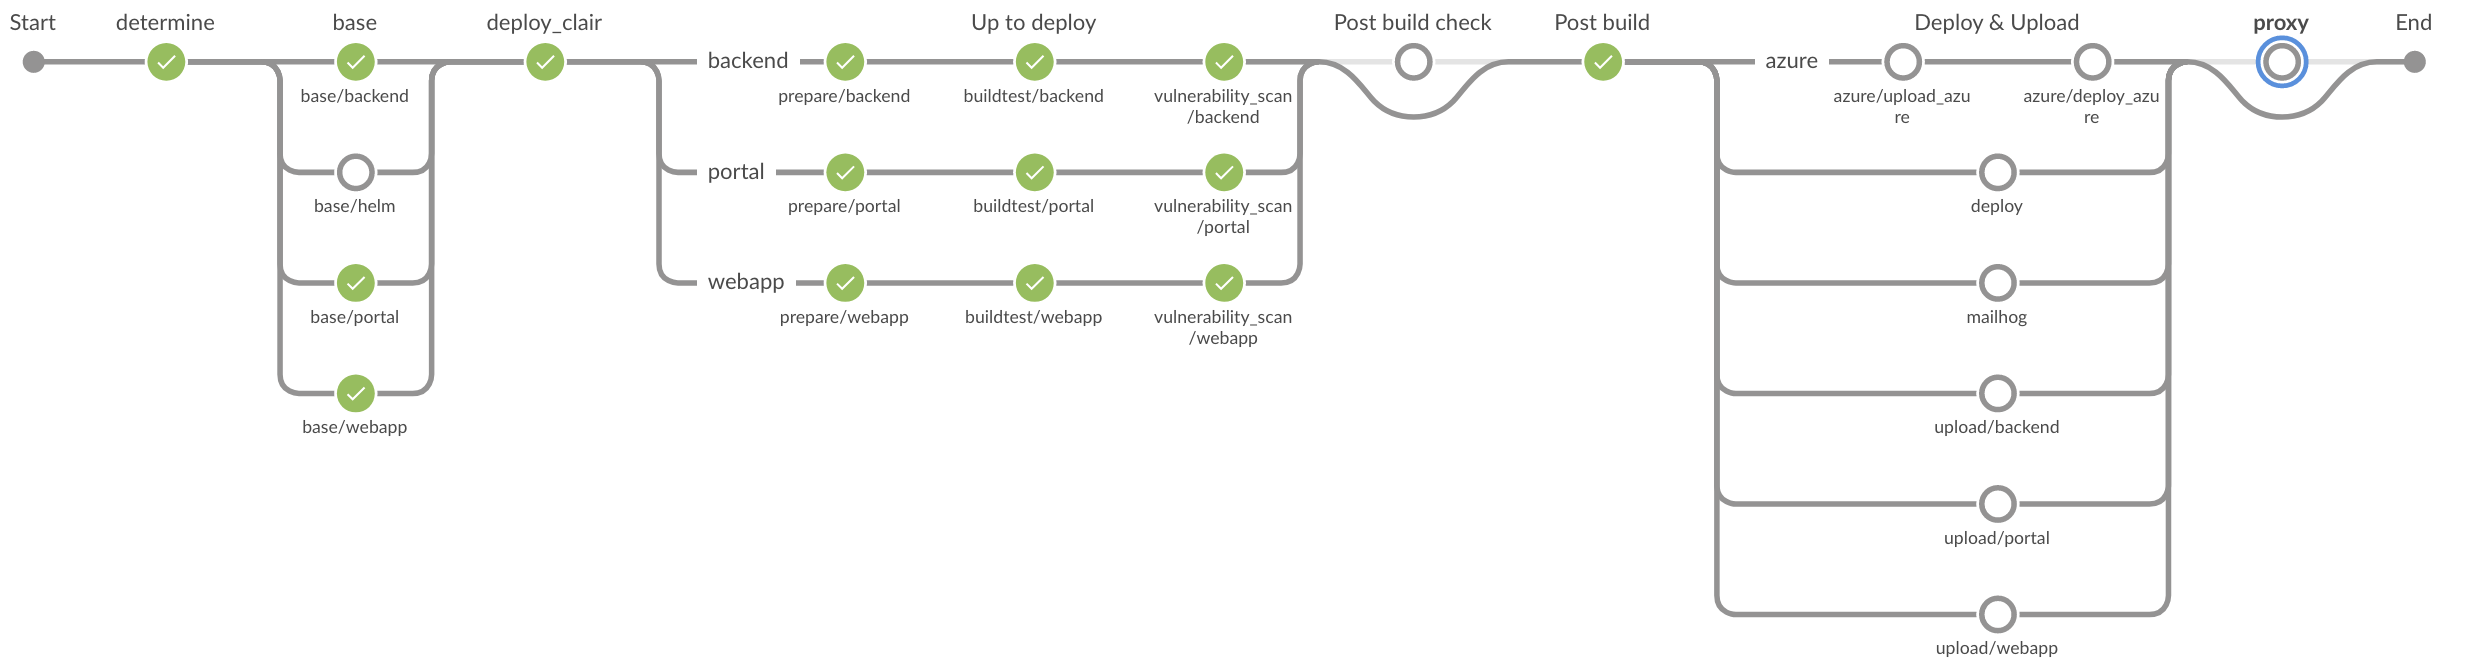
\includegraphics[width=15cm]{gfx/Screenshot 2021-08-18 Jenkins PipeLine}
\caption{Jenkins(Blue Ocean) pipeline}
\label{fig:JenkinsPipeLine}
\end{figure}
Een Jenkins pipeline werkt in een aantal stappen dat in een .jenkinsFile wordt beschreven.
Deze jenkinsFile wordt in de determine stap ingelezen en de benodigde stappen op een rij gezet.
De stappen die worden uitgevoerd zijn:
\begin{itemize}
\item \textbf{determine} Nu wordt bekeken welke stappen er nodig zijn om een succesvolle build en of deploy te kunnen doen./ Aan de hand van een JenkinsFile en tokens in een Commit message wordt hier bekeken welke stappen er moeten worden uitgevoerd om tot een goed einde te komen.
\item \textbf{base} In de base stap worden alle Containers voorbereid die nodig zijn om de applicatie te draaien.\ Images worden opgehaald en gedeployed De base stap is een parallel lopende stap waarin in dit geval backend, portal en de app worden voorbereid.
\item \textbf{deploy clair} de clair scanner zoekt op kwetsbaarheden binnen containers die zojuist zijn aangemaakt.\ Dit is een extra veiligheid die ervoor zorgt dat de images en container veilig zijn er alleen nog door bibliotheken die gebruikt worden voor ontwikkeling kwetsbaarheden kunnen worden toegevoegd
\item \textbf{Up to deploy}
in dit geval wordt er voor de backend, portal, en app een parallel process gestart waarin alle drie substappen doorlopen:
\begin{itemize}
\item \textbf{prepare} Docker containers worden ingesteld, en klaar gezet voor het ontvangen van de services.
\item \textbf{builtest} De services worden gebuild en gestest in deze stap.\ Eaglescience heeft een aantal tresholds opgesteld waaraan tests moeten voldoen om deze te analyseren worden de test resultaten vanuit de docker containers gekopieerd naar de Jenkins Store waar Jenkins de waarden kan analyseren als alle tests binnen de resultaten vallen wordt de volgende stap uitgevoerd.
\item \textbf{vulnerability scan} Clair scanner scant nu de containers nogmaals maar nu op de gebruikte software.\ Als clair iets vind dat eaglescience als verdacht acht dan wordt de build gestaakt.
\end{itemize}
\item \textbf{PostBuild(check)}
Alle bevindingen worden hier gecheckt mocht er iets mis zijn wordt er wederom afgebroken en is de build gefaald en kan er dus niet een deploy plaatsvinden.
\item \textbf{Deploy \& Upload}
in dit geval wordt de deploy niet uitgevoerd.\ Deze stap zorgt ervoor dat de gebouwde containers worden overgedragen naar Azure.\ Iedere container heeft wederom zijn eigen stappen.
\item \textbf{End}
Einde van de PipeLine Jenkins geeft de workers die het project heeft gebruikt weer vrij.
\end{itemize}
